\en{In this chapter, we define the "quasiperiods" of a lattice with help of the Weierstraß $\zeta$-function.
We also give an alternative representation of the periods and quasiperiods with help of elliptic integrals.
For this, we use the algebraic differential equation of $\wp$ from Prop.~\ref{\en{EN}dglP}.}%
\de{In diesem Abschnitt definieren wir den Begriff \glqq Quasiperiode\grqq~eines Gitters mit Hilfe der Weierstraß'schen $\zeta$-Funktion und geben eine alternative Darstellung der Perioden und Quasiperioden mit Hilfe elliptischer Integrale an. Hierfür benötigen wir die Differentialgleichung der $\wp$-Funktion aus Satz~\ref{\en{EN}dglP}.}

\begin{thm}\label{\en{EN}eta}
\en{The Weierstraß $\zeta$-function from Def.~\ref{\en{EN}defizeta} is not doubly periodic, but the following value of the "quasiperiod"}%
\de{Die Weierstraß'sche $\zeta$-Funktion aus Def.~\ref{\en{EN}defizeta} ist zwar nicht doppeltperiodisch, aber immerhin ist der Wert der \glqq Quasiperiode\grqq}
$$\eta(\omega;L):=\zeta(z+\omega;L)-\zeta(z;L)$$
\en{is independent of the choice of $z$ (as long as $z\notin L$).}%
\de{unabhängig von der Wahl von $z$ (solange $z\notin L$).}
\end{thm}
\begin{proof}
\en{If we call the right hand side $R(z):=\zeta(z+\omega;L)-\zeta(z;L)$ and derive by $z$, we get from Def.~\ref{\en{EN}defiwp} that $R'(z)=-\wp(z+\omega;L)-(-\wp(z;L))=\wp(z;L)-\wp(z+\omega;L)$.
Prop.~\ref{\en{EN}wpdoppeltper} tells us that this is zero, so $R(z)$ is constant with respect to $z$.
The value of this constant thus depends only on the lattice $L$ and on the choice of $\omega$ -- and we can call it $\eta(\omega;L)$.}%
\de{Wenn wir die rechte Seite mit $R(z):=\zeta(z+\omega;L)-\zeta(z;L)$ bezeichnen und nach $z$ ableiten, erhalten wir nach Def.~\ref{\en{EN}defiwp}: $R'(z)=-\wp(z+\omega;L)-(-\wp(z;L))=\wp(z;L)-\wp(z+\omega;L)$.
Nach Satz~\ref{\en{EN}wpdoppeltper} ist das Null, also ist $R(z)$ konstant bezüglich $z$. Diese Konstante hängt dann noch vom Gitter $L$ und von der Wahl von $\omega$ ab -- und wir können sie mit $\eta(\omega;L)$ bezeichnen.}
\end{proof}

\begin{defi}\label{\en{EN}defetak}
\en{The following values $\eta_1(L)$ and $\eta_2(L)$ are called "basic quasiperiods" of the lattice $L=\mathbb Z \omega_1 + \mathbb Z \omega_2$:}%
\de{Man nennt die folgenden Werte $\eta_1(L)$ und $\eta_2(L)$ auch \glqq Basis-Quasi"-perioden\grqq~ des Gitters $L=\mathbb Z \omega_1 + \mathbb Z \omega_2$:}
$$\eta_k(L):=\zeta(z+\omega_k;L)-\zeta(z;L)$$
\en{Remark: by applying Prop.~\ref{\en{EN}eta} repeatedly, we see that these two values generate all other quasiperiods $\eta(\omega;L)$ like a lattice -- this is the reason they are called "basic" quasiperiods.}%
\de{Bemerkung: durch wiederholte Anwendung der Beziehung aus Satz~\ref{\en{EN}eta} folgt, dass diese beiden Werte sämtliche anderen Quasiperioden $\eta(\omega;L)$ wie ein Gitter erzeugen, deshalb heißen sie \glqq Basis\grqq-Quasiperioden.}
\end{defi}


\begin{bem}\label{\en{EN}bempitch}
\en{In Def.~\ref{\en{EN}defetak} we see that $\eta_k$ gives the difference in the value of the $\zeta$-function if the argument is changed by $\omega_k$.
The commonly used terms "period of the lattice" and "quasiperiod of the lattice" are thus a bit inappropriate or misleading:
\begin{itemize}
    \item Instead of "period of the lattice $L$", $\omega_k$ should be called "period of the associated $\wp$-function".
    \item Instead of "quasiperiod of the lattice $L$", $\eta_k$ should be called "pitch of the associated $\zeta$-function" (cf.~"pitch of a helix").
\end{itemize}
Anyway, we will continue with the commonly used terms.}%
\de{In Definition~\ref{\en{EN}defetak} erkennen wir, dass $\eta_k$ angibt, um wie viel der Wert der $\zeta$-Funktion zunimmt, wenn man das Argument um $\omega_k$ verändert.
Die in der Literatur üblichen Begriffe \glqq Periode des Gitters\grqq~und \glqq Quasiperiode des Gitters\grqq~sind also eigentlich unpassend:
\begin{itemize}
    \item Für $\omega_k$ sollte man statt \glqq Periode des Gitters $L$\grqq~besser \glqq Periode der $\wp$-Funktion zum Gitter $L$\grqq~sagen.
    \item Für $\eta_k$ sollte man statt \glqq Quasiperiode des Gitters $L$\grqq~besser \glqq Gewindesteigung oder Ganghöhe der $\zeta$-Funktion zum Gitter $L$\grqq~sagen.
\end{itemize}
Wir werden trotzdem die üblichen Begriffe weiter verwenden.}
\end{bem}


\begin{thm}[\en{Legendre's relation}\de{Legendre'sche Relation}]\label{\en{EN}legendre}
\en{For the basic periods and the associated basic quasi\-periods of a lattice $L=\mathbb Z \omega_1 + \mathbb Z \omega_2$ it holds:}%
\de{Für die Basisperioden und zugehörigen Basisquasiperioden des Gitters $L=\mathbb Z \omega_1 + \mathbb Z \omega_2$ gilt die sogenannte \glqq Legendre'sche Relation\grqq :} $$\eta_1\omega_2-\eta_2\omega_1 = 2\pi i$$
\end{thm}
\begin{proof}
\en{We shift the fundamental parallelogram $\overline{\mathcal P}$ (Def.~\ref{\en{EN}fund}), so that there are no lattice points on the border of $\overline{\mathcal P}_v=\overline{\mathcal P}+v$ with $v\in\mathbb C$. Then the residue theorem yields}%
\de{Wir verschieben das Periodenparallelogramm $\overline{\mathcal P}$ (Def.~\ref{\en{EN}fund}) so, dass keine Gitterpunkte auf dem Rand liegen: $\overline{\mathcal P}_v=\overline{\mathcal P}+v$ mit $v\in\mathbb C$. Dann liefert der Residuensatz:}
$$\oint_{\delta\overline{\mathcal P}_v} \zeta(z)dz = 2 \pi i,$$
\en{because the $\zeta$-function has (modulo $L$) only one pole with residue $1$ (see Def.~\ref{\en{EN}defizeta}).
On the other hand one can combine the values of the integrals along opposite sides (using Def.~\ref{\en{EN}defetak}):
The sides parallel to $\omega_1$ contribute $-\eta_2\omega_1$, the sides parallel to $\omega_2$ contribute $\eta_1\omega_2$. In total, the value of the integral is $\eta_1\omega_2-\eta_2\omega_1 = 2\pi i$.}%
\de{weil die $\zeta$-Funktion (modulo $L$) nur einen Pol mit Residuum $1$ hat (siehe Def.~\ref{\en{EN}defizeta}).
Andererseits kann man unter Verwendung der Definition~\ref{\en{EN}defetak} der Quasiperioden die Integrale längs gegenüberliegender Kanten zusammenfassen: die beiden zu $\omega_1$ parallelen Kanten liefern einen Beitrag von $-\eta_2\omega_1$, die beiden zu $\omega_2$ parallelen Kanten liefern $\eta_1\omega_2$.
Insgesamt lautet der Wert des Integrals also $\eta_1\omega_2-\eta_2\omega_1 = 2\pi i$.}
\end{proof}

\begin{defi}\label{\en{EN}defX}
\en{Let $g_2$ and $g_3$ be two complex numbers. Then}%
\de{Seien $g_2$ und $g_3$ zwei komplexe Zahlen. Dann ist}
$$X(g_2,g_3) := \left\{\left.(x,y)\in\mathbb C^2~\right|~y^2 = 4x^3 - g_2 x - g_3\right\}$$
\en{is an example of a "plane affine algebraic curve". Given a lattice $L$, we use $g_2=g_2(L)$ and $g_3=g_3(L)$ as in Prop.~\ref{\en{EN}dglP} and obtain:}%
\de{ein Beispiel einer \glqq ebenen affinen Kurve\grqq. Wenn ein Gitter $L$ gegeben ist, dann kann man mit $g_2=g_2(L)$ und $g_3=g_3(L)$ aus Satz~\ref{\en{EN}dglP} auch schreiben:}
$$X(L)=X(g_2(L),g_3(L))$$
\end{defi}

\begin{thm}\label{\en{EN}EbeneAffineKurve}
\en{The mapping $\Phi$ with}%
\de{Die Zuordnung $\Phi$ mit}
$$\begin{aligned}
\Phi: \mathbb C - L~& \to~  X(g_2(L),g_3(L))\subset\mathbb C^2\\
 z ~~~~&\mapsto~ (\wp(z;L),\wp'(z;L))
\end{aligned}$$
\en{is well-defined, differentiable and doubly periodic.}%
\de{ist wohldefiniert, differenzierbar und doppeltperiodisch.}
\end{thm}
\begin{proof}
\en{From the differential equation of the $\wp$-function (Prop.~\ref{\en{EN}dglP}) and the compatible definition of $X(g_2(L),g_3(L))$ we get that $\Phi$ is well-defined.
Since both $\wp$ and $\wp'$ are doubly periodic and differentiable, the same holds for $\Phi$.}%
\de{Die Wohldefiniertheit folgt aus der algebraischen Differentialgleichung der $\wp$-Funk"-tion in Satz~\ref{\en{EN}dglP} und der dazu passend gewählten Definition von $X(g_2(L),g_3(L))$. $\Phi$ ist doppeltperiodisch und differenzierbar, weil sowohl $\wp$ als auch $\wp'$ doppeltperiodisch und differenzierbar sind.}
\end{proof}

\begin{defi}\label{\en{EN}defwege}
\en{Let $L=\mathbb Z \omega_1 + \mathbb Z \omega_2$ be a lattice with basic periods $\omega_1$ and $\omega_2$. Then we define the paths $\beta_1$ and $\beta_2$ as follows:}%
\de{Es sei $L=\mathbb Z \omega_1 + \mathbb Z \omega_2$ ein Gitter mit Basisperioden $\omega_1$ und $\omega_2$. Dann definieren wir die beiden Wege $\beta_1$ und $\beta_2$ wie folgt:}
\begin{align*}
    \beta_1(t):=\frac 1 4 \cdot \omega_2 + t \cdot \omega_1 \qquad\text{\en{for}\de{für}~ } 0\leq t\leq 1\\
    \beta_2(t):=\frac 1 4 \cdot \omega_1 + t \cdot \omega_2 \qquad\text{\en{for}\de{für}~ } 0\leq t\leq 1
\end{align*}
\end{defi}

\begin{bem}\label{\en{EN}bemwege}
\en{The paths $\beta_k$ from Def.~\ref{\en{EN}defwege} are shown in Fig.~\ref{\en{EN}abbwege}.
On these paths, there are no poles of $\wp$ and $\wp'$ (black dots in the figure) and no zeros of $\wp'$ (circles in the figure, cf.~Prop.~\ref{\en{EN}zerowp}).}%
\de{Die in~\ref{\en{EN}defwege} definierten Wege $\beta_k$ sind in Abbildung~\ref{\en{EN}abbwege} zu sehen.
Auf den Wegen liegen keine Polstellen von $\wp$ und $\wp'$ (schwarze Punkte im Bild); und keine Nullstellen von $\wp'$ (Kreise im Bild, vgl.~Satz~\ref{\en{EN}zerowp}).}



\begin{figure}[ht]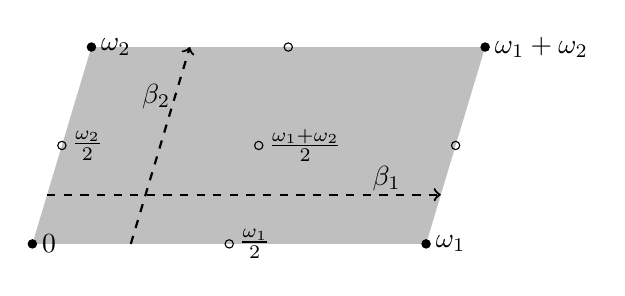
\begin{tikzpicture}[x=25mm, y=25mm] 
   \path[fill=lightgray] (0,0) -- (2,0) -- (2.3,1) -- (0.3,1) -- cycle;
   \draw[fill=black] (0,0) circle (1.5pt) node[right] {$0$};
   \draw[fill=black] (2,0) circle (1.5pt) node[right] {$\omega_1$};
   \draw[fill=black] (0.3,1) circle (1.5pt) node[right] {$\omega_2$};
   \draw[fill=black] (2.3,1) circle (1.5pt) node[right] {$\omega_1+\omega_2$};
   \draw             (0.15,0.5) circle (1.5pt) node[right] {$\frac{\omega_2}{2}$};
   \draw             (1.15,0.5) circle (1.5pt) node[right] {$\frac{\omega_1+\omega_2}{2}$};
   \draw             (1,0) circle (1.5pt) node[right] {$\frac{\omega_1}{2}$};
   \draw             (2.15,0.5) circle (1.5pt);
   \draw             (1.3,1) circle (1.5pt);
   \draw[->,dashed,thick] (0.075,0.25) -- (2.075,0.25) ;
   \draw[->,dashed,thick] (0.5,0) -- (0.8,1) ;
   \draw (1.8,0.22) node[above] {$\beta_1$};
   \draw (0.75,0.75) node[left] {$\beta_2$};
\end{tikzpicture}
\caption{\en{Fundamental parallelogram $\overline{\mathcal P}$ (cf.~Def.~\ref{\en{EN}fund}) with lattice points (poles of $\wp$ and $\wp'$) and half lattice point (zeros of $\wp'$) and paths $\beta_k$ from Def.~\ref{\en{EN}defwege}.}%
\de{Periodenparallelogramm $\overline{\mathcal P}$ (vgl.~Def.~\ref{\en{EN}fund}) mit Gitterpunkten (Polstellen von $\wp$ und $\wp'$) und halben Gitterpunkten (Nullstellen von $\wp'$) und den Wegen $\beta_k$ aus Def.~\ref{\en{EN}defwege}.}}\label{\en{EN}abbwege}
\end{figure}
\end{bem}

\begin{thm}\label{\en{EN}satzint}
\en{Let}\de{Es sei} $L=\mathbb Z \omega_1 + \mathbb Z \omega_2$.
\en{Then we use the paths $\beta_k$ from Def.~\ref{\en{EN}defwege} to define two new paths $\alpha_k:=(\wp(\beta_k),\wp'(\beta_k))$.
These $\alpha_k$ are closed paths in the plane affine algebraic curve $X(g_2(L),g_3(L))$.
Here, the basic periods and basic quasiperiods of the lattice admit the following representation by elliptic integrals:}%
\de{Dann definieren wir mit Hilfe der Wege $\beta_k$ aus Def.~\ref{\en{EN}defwege} zwei Wege $\alpha_k:=(\wp(\beta_k),\wp'(\beta_k))$.
Diese $\alpha_k$ sind geschlossene Wege durch die ebene affine Kurve $X(g_2(L),g_3(L))$.
Die Basisperioden bzw.~Basisquasiperioden des Gitters kann man dann durch die folgenden elliptischen Integrale darstellen:}
\begin{align*}
    \omega_k = \oint_{\alpha_k} \frac{dx}{y} \qquad \text{ \en{and}\de{sowie} }\qquad \eta_k(L)  = -\oint_{\alpha_k} \frac{x~dx}{y}
\end{align*}
\end{thm}
\begin{proof}\belowdisplayskip=-12pt
\en{The paths $\alpha_k$ are indeed paths in $X(g_2(L),g_3(L))$, because the differential equation from Prop.~\ref{\en{EN}dglP} guarantees, that the equation from Def.~\ref{\en{EN}defX} is fulfilled everywhere on $\alpha_k$.
From $\beta_k(1)=\beta_k(0)+\omega_k$ we deduce $\wp(\beta_k(0))=\wp(\beta_k(1))$ and the same for $\wp'$. Thus it holds $\alpha_k(0)=\alpha_k(1)$ and the paths $\alpha_k$ are closed.
With $(x,y)=(\wp(z),\wp'(z))$ along the paths $\alpha_k$ we get $\frac{dx}{dz}=\wp'(z)$ and thus}%
\de{Die Wege $\alpha_k$ sind tatsächlich Wege durch $X(g_2(L),g_3(L))$, weil mit der Differentialgleichung der $\wp$-Funktion (Satz~\ref{\en{EN}dglP}) folgt, dass die definierende Gleichung aus Def.~\ref{\en{EN}defX} für alle Punkte auf $\alpha_k$ erfüllt ist.
Aus $\beta_k(1)=\beta_k(0)+\omega_k$ folgt $\wp(\beta_k(0))=\wp(\beta_k(1))$ und Gleiches für $\wp'$. Also ist $\alpha_k(0)=\alpha_k(1)$ und somit sind die Wege $\alpha_k$ geschlossen.
Mit $(x,y)=(\wp(z),\wp'(z))$ entlang der Wege $\alpha_k$ folgt dann $\frac{dx}{dz}=\wp'(z)$ und somit}
\begin{align*}
    \oint_{\alpha_k} \frac{dx}{y}
    &=\int_{\beta_k}\frac{\wp'(z)dz}{\wp'(z)}
    =\int_{\beta_k} dz = \beta_k(1)-\beta_k(0) = \omega_k\\
    \text{\en{and}\de{und}}\qquad-\oint_{\alpha_k} \frac{x~dx}{y}
    &=-\int_{\beta_k}\frac{\wp(z)\wp'(z)dz}{\wp'(z)}
    =\int_{\beta_k} -\wp(z) dz\\
    &=\int_{\beta_k} \zeta'(z) dz
    = \zeta(z+\omega_k;L)-\zeta(z;L) = \eta_k(L)
\end{align*}
\end{proof}
